\documentclass[12pt,a4paper]{report}
\usepackage[pdftex]{graphicx} 
\renewcommand{\baselinestretch}{1.5}
%\usepackage{url} %for proper url entries
\usepackage[bookmarks, colorlinks=false, pdfborder={0 0 0}, pdftitle={Techniques to Secure Data on Cloud: Docker Swarm or Kubernetes?}, pdfsubject={<subject here>}, pdfkeywords={<keywords here>}]{hyperref} %for creating links in the pdf version and other additional pdf attributes, no effect on the printed document
%\usepackage[final]{pdfpages} %for embedding another pdf, remove if not required
\usepackage{geometry}
\usepackage[pdftex]{graphicx}
\usepackage{graphicx}
\usepackage{amsmath}
\usepackage{fixltx2e}
\usepackage{multirow}
\usepackage{textcomp}

\geometry{
	left=2.2cm,
	top=2.54cm,
	bottom=2.921cm,
	right=1.5cm
}
\usepackage{fancyhdr}
\pagestyle{fancy}
\fancyhead [L]{}
\lfoot{\textit{Department of Computer Applications,CET}}


\renewcommand{\headrulewidth}{0.4pt}
\renewcommand{\footrulewidth}{0.4pt}

\begin{document}
\begin{titlepage}
\begin{center}
\textbf{ A  }\\
\vspace{0.35cm}
\textbf{ Seminar Report}\\
\vspace{0.35cm}
\textbf{ On  }\\
\vspace{0.55cm}
\textbf{\Large{Techniques to Secure Data on Cloud: Docker Swarm or Kubernetes?}}\\ \vspace{0.5 cm}
\normalsize
\vspace{0.5cm}
\emph{Submitted in partial fulfillment of the requirements for the Award of the Degree}\\
\vspace{0.35cm}
\emph{of}\\
\vspace{0.35cm}
Master of Computer Applications\\
\vspace{0.35cm}
%in\\
%\vspace{0.35cm}
%Computer Science and Engineering(Image processing)\\
%\vspace{0.35cm}
\emph{of}\\
\vspace{0.35cm}
\emph{ {APJ Abdul Kalam Technological University} }\\
\normalsize
\vspace{0.5cm}

\includegraphics[height=0.30\textwidth]{1-title/images/cet.jpg}\\
\vspace{0.3cm}
Submitted by\\
\vspace{0.3cm}
\textbf{SASHWAT K}\\
\vspace{0.5cm}
\textbf{TVE17MCA042 }\\
\vspace{1.0cm}

\normalsize
\textbf{Department of Computer Applications}\\[0.3cm]
\textbf{COLLEGE OF ENGINEERING, TRIVANDRUM}\\[0.4cm]
\textbf{NOVEMBER 2019}\\
\end{center}
\end{titlepage}



\begin{titlepage}
\begin{center}
\textbf{DEPARTMENT OF COMPUTER APPLICATIONS}\\[0.5cm]
\textbf{ COLLEGE OF ENGINEERING TRIVANDRUM}\\
[0.5cm]
\vspace{1.2cm}

\includegraphics[width=0.30\textwidth]{1-title/images/cet.jpg}\\
\vspace{0.8cm}
\textbf{CERTIFICATE}\\
%\normalsize
\end{center}
%\normalsize
\emph{Certified that this Seminar report entitled,\textbf{``Techniques to Secure Data on Cloud: Docker Swarm or Kubernetes?"} is the paper presented by \textbf{"Sashwat K" (Reg No: TVE17MCA042)} in partial fulfillment of the requirements for the award of the degree of Master of Computer Applications of APJ Abdul Kalam Technological University during the year 2019.}\\\\\\\\
\vspace{0.9cm}
Prof. Jose T Joseph.
\hspace{9.3cm}
Dr. Sabitha S.\\ 
\hspace{5cm}
 \textbf{Co-ordinator}
\hspace{9cm}
%\hspace{0.5cm}
\textbf{Head of the Department}

\end{titlepage}

\begin{titlepage}
\begin{center}
\textbf{\LARGE{Acknowledgement}}\\[0.5cm] 
\end{center}
\paragraph{\hspace{1cm}}
First and for most I thank \textbf{GOD} almighty and to my parents for the success of this seminar. I owe a sincere gratitude and heart full thanks to everyone who shared their precious time and knowledge for the successful completion of my seminar.
\paragraph{\hspace{1cm}}
I would like to thank \textbf{Dr Jiji C V}, Principal,  College of Engineering Trivandrum, who helped me during the entire process of work.
\paragraph{\hspace{1cm}}
I am extremely grateful to \textbf{Prof.Sabitha S}, HOD, Dept of Computer Applications, for providing me with best facilities and atmosphere for the creative work guidance and encouragement.
\paragraph{\hspace{1cm}}
I would like to thank my coordinator,\textbf{ Prof.Jose T Joseph}, Dept of Computer Applications, who motivated me throughout the work of my seminar.  
\paragraph{\hspace{1cm}}
I profusely thank other Asst. Professors in the department and all other staffs of CET, for their guidance and inspirations throughout my course of study.
\paragraph{\hspace{1cm}}
I owe my thanks to my friends and all others who have directly or indirectly helped me in the successful completion of this seminar. No words can express my humble gratitude to my beloved parents and relatives who have been guiding me in all walks of my journey.\\

 \vspace{1.1cm}
\hspace{345pt} \textbf{Sashwat K}


\end{titlepage}

\begin{abstract}
\paragraph{\hspace{24pt}}
In the current world with immense technological advancement, the Information Technology(IT) world is switching from physical storage to cloud storage since the “cloud” providers supply resources on demand over the Internet. Cloud computing is a successful and speedy evolving model with new features and capabilities being announced regularly. The concept of this is known as “pay as you use” which enables the firms to shift to cloud. Due to this, security of such data has become an issue. Security of cloud-based applications is one of the key concerns of cloud customers. These three principles of cloud security are Availability, Confidentiality and Integrity. One of the most efficient ways is with the help of Container Clustering. There are various ways in which container clustering can be achieved. This paper presents the study and the comparison between two such technologies, i.e. Docker Swarm and Kubernetes.
\end{abstract} 

\pagenumbering{roman} %numbering before main content starts
\tableofcontents
\listoffigures
\newpage
\pagenumbering{arabic}
\chapter{Introduction}

\paragraph{\hspace{24pt}}
“A Cloud Computing model is a model which enables convenient, on demand network access to a shared pool of configurable computing resources and services. These resources include: networks, servers, storage, apps and services. These resources can be rapidly provisioned and released with minimal management effort or service provider interaction.”Cloud provides portability and flexibility of online services.

\paragraph{\hspace{24pt}}Introduction continues from 1.1 to 1.5. Chapter 2 of this paper discusses the key concerns of Data Security on Cloud. Chapter 3 discusses the various Issues. Chapter 4 discusses the Various Techniques to Secure Data on Cloud. Chapter 5 to 8 discuss about container clustering using docker and its working. Chapter 9 and 10 discuss about Kubernetes and why it is better than Docker Swarm.

\begin{figure}[htb]
\centering
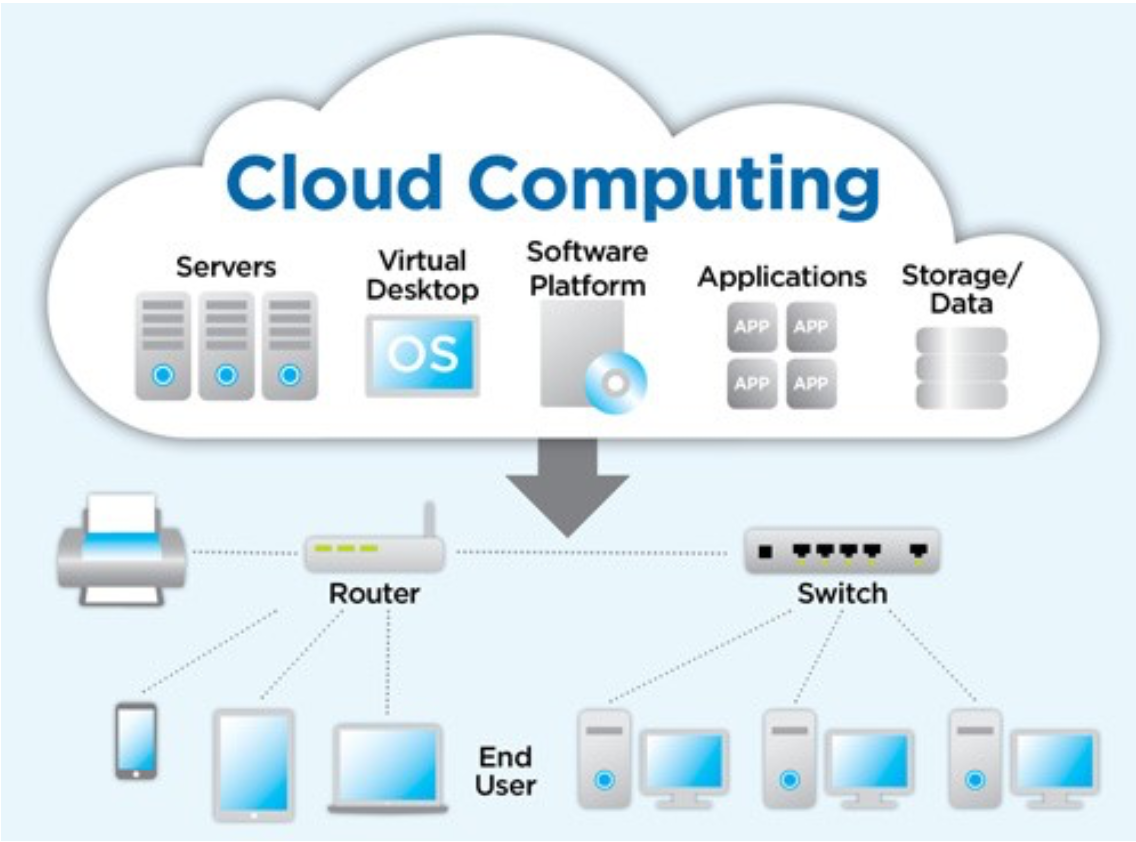
\includegraphics[width=10cm,height=6cm]{5-contents/1-Introduction/images/cloud-computing-intro.png} % e.g. insert ./image for image.png in the working directory, adjust scale as necessary
\caption{Cloud Computing}
\label{fig:label} % insert suitable label, this is used to refer to a fig from within the text as shown above
\end{figure}

\section{The Five Essential Characteristics}
\paragraph{\hspace{24pt}}
The Five essential characteristics of Cloud Computing are given below. These are vital features of this technology which define its usability and efficiency.\\
\textbf{1. On-Demand Self Service} {“A consumer can one-sidedly provision computing capabilities. These capabilities include server time and network storage. They can be provisioned whenever required without having human interaction with the service providers.”}\\
\textbf{2. Broad Network Access} {here are capabilities available over the network and can be accessed through various platforms such as mobile phones, laptops, PDAs and other electronic devices.}\\
\textbf{3. Resource Pooling} {The resources are amalgamated to serve multiple customers. This can be done with the help of multi-tenant models. These resources are dynamically assigned and reassigned depending on the consumer’s demands. Examples of such resources include storage, Memory, Processing, Network, Bandwidth and Virtual Machines.}\\
\textbf{4. Rapid Elasticity} {The capabilities can be provided elastically and rapidly, sometimes also automatically, for quick scale outs, and rapid releases to quickly scale in to the customer. Such capabilities are unlimited and can be bought whenever needed and in any quantity.}\\
\textbf{5. Measured Service} {The use of resources in cloud systems are automatically controlled and optimised. The usage of the services can be monitored and controlled. They can also be reported providing transparency for both, the provider and consumer.}

\section{The Three Service Models}
\paragraph{\hspace{24pt}}
There are three service models which are implanted in Cloud Computing. They are as follows:\\
\textbf{1. Infrastructure as a Service(IaaS)} {In IaaS, the consumer is provided with networks, storage, processing and various other computing resources. IaaS enables he consumer or user to deploy and execute the software. This software includes OSs and applications. The consumer is not in control of the cloud infrastructure. However, a consumer can control the OS, storage and the deployed apps. A consumer may also have partial control over selection of networking components such as host firewalls.}\\
\textbf{2. Platform as a Service (PaaS)} {PaaS allows the consumers to deploy their applications which are created using programming languages and various tools onto the cloud infrastructure. The control that the consumer has is similar to that of IaaS.}\\
\textbf{3. Software as a Service (SaaS)} {SaaS enables the consumer to use the capabilities such as applications which is provided by the service provider which runs on the infrastructure. These applications can be accessed from various devices through a thin client interface such as a web browser like Google Chrome, Mozilla Firefox, IE, Opera etc. The control that the consumer has is similar to that of IaaS and PaaS. However, the consumer may have partial control over user specific application configuration settings.}

\section{The Four Deployment Models}
\paragraph{\hspace{24pt}}
The cloud can be deployed in four different ways. They are as follows:\\

\begin{figure}[htb]
\centering
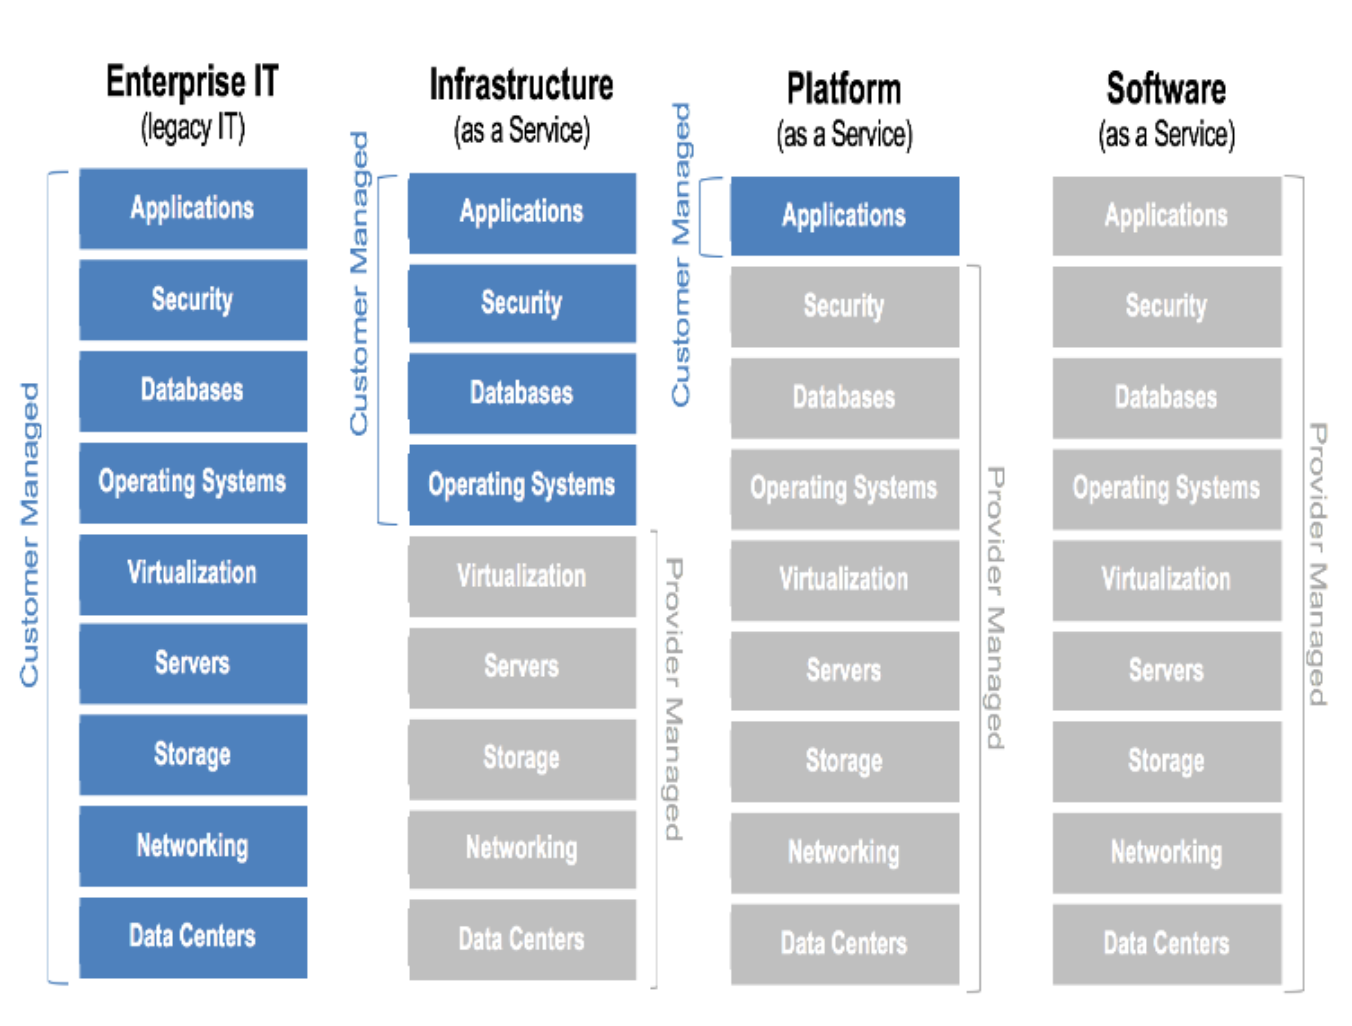
\includegraphics[width=12cm,height=8cm]{5-contents/1-Introduction/images/service-model.png} % e.g. insert ./image for image.png in the working directory, adjust scale as necessary
\caption{The Service Models}
\label{fig:label} % insert suitable label, this is used to refer to a fig from within the text as shown above
\end{figure}

\textbf{1. Public Cloud} {As the name suggests, this type of cloud is available to the general public. It is owned by organizations that sell cloud services. These service providers include Amazon’s Elastic Compute Cloud(EC2), Microsoft Azure Service Platform, Sun Cloud, Google App Engine, IBM’s Blue Cloud, etc.}\\
\textbf{2. Private Cloud} {This cloud infrastructure is operated solely for an organization. “The objective of a private cloud is not sell as-a-service offerings to external customers but to gain the benefits of cloud architecture without giving up the control of maintaining your own data centre.” A particular private cloud can be owned only by a single entity or organization.}\\
\textbf{3. Community Cloud} {The infrastructure of the community cloud is shared by multiple organizations. It supports a specific community that has similar or same concerns/issues. It may be managed by the organizations or a third party.}\\
\textbf{4. Hybrid Cloud} {A hybrid cloud is the incorporation of two or more clouds. Hybrid clouds can remain as unique entities. However, they are bound together by standardized technology that enables portability of data and applications.}
Users may use any of the deployment models as per their requirements and needs.

\begin{figure}[htb]
\centering
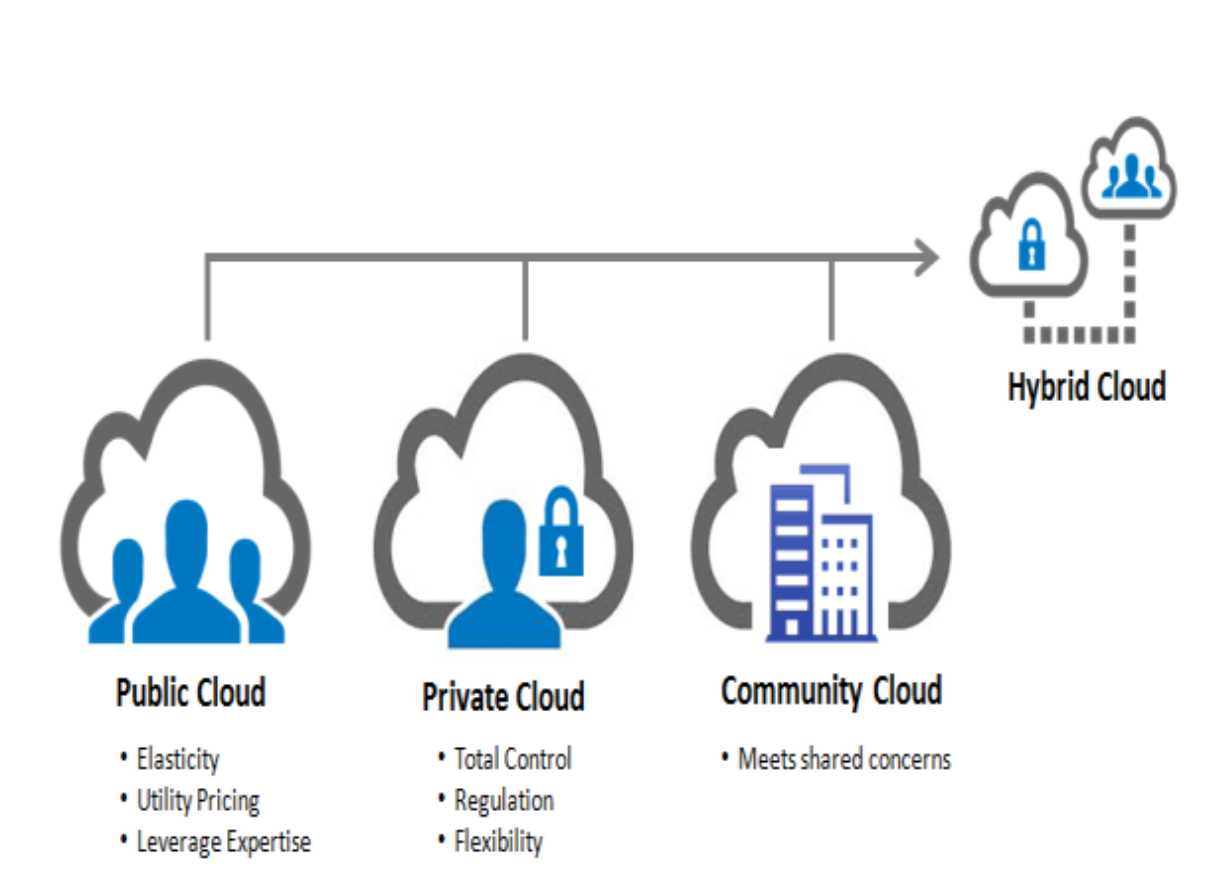
\includegraphics[width=12cm,height=8cm]{5-contents/1-Introduction/images/cloud-computing-model.png} % e.g. insert ./image for image.png in the working directory, adjust scale as necessary
\caption{Cloud Computing Models}
\label{fig:label} % insert suitable label, this is used to refer to a fig from within the text as shown above
\end{figure}

\section{Pros and Cons of Computing}
\paragraph{\hspace{24pt}}
Every technology has its own advantages and disadvantages. The pros and cons of Cloud Computing are as given below.

\subsection{Advantages}
\begin{enumerate}
    \item Minimized Costs
    \item Higher Resource Sharing.
    \item Consumption based cost.
    \item Efficient power saving.
    \item Faster time to deploy new services.
    \item Management moves to Cloud Provider
\end{enumerate}

\subsection{Disadvantages}
\begin{enumerate}
    \item Reliability
    \item Availability
    \item Security and Privacy Latency and Bandwidth guarantees.
    \item Absence of robust SLAs
    \item Uncertainty around inter-operablity, portability and lock-in.
    \item Compliance/Regulatory Laws mandate on-site ownership of data.
\end{enumerate}

\paragraph{\hspace{24pt}}
There are various advantages and disadvantages of Cloud Computing. Users must keep them in mind when they choose Cloud Computing for installing their applications or storing their data on Cloud servers.
\chapter{Data Security, its Issues and Various Methods of Data Security}

\paragraph{\hspace{24pt}}
Data security is one of the key concerns with Cloud Computing. Data security has three major factors to be considered. Security refers to the availability, integrity and confidentiality of data. Not providing or guaranteeing this may pose major issues for cloud vendors.\\\\

\textbf{Availability} {It is one of the most problematic issue faced by the consumers. Most cloud vendors have experienced downtime of their services which have affected majority of the users of cloud services. For example, Amazon servers have faced such issues which have been said to be Denial of Service attack. A cloud server must be available at all times and if not, a particular time period should be given as notice for the services to resume.}\\

\textbf{Integrity} {This is another important feature as cloud vendor or provider must provide. Data integrity refers to the accuracy and consistency of data stored on the cloud or any database as a matter of fact. Thin clients can be used to maintain integrity of data or security of data on the client side. This is possible since thin clients use as few resources as possible and they do no store any data. By doing this, personal information such as passwords cannot be stolen.}\\

\textbf{Confidentiality} {Personal or confidential data stored on the cloud should not be accessible by anyone other than the authorised entity. For example, data from parent company X which has been stored in child company Y should not be accessible by the employees of company Y, since it is confidential data of company X.}

\paragraph{\hspace{24pt}}
These are the factors essential for Data Security in any kind of network platform. Guaranteeing the mentioned factors ensures the security of the consumers or customers data.

\paragraph{\hspace{24pt}}
There are various issues that require addressing before an organization or enterprise considers switching to the cloud computing model. These issues are Privileged User Access, Data Location, Recovery, Long- term Viability, Data Segregation and Regulatory Compliance.

\paragraph{\hspace{24pt}}
The below mentioned graph shows the issues or concerns and its corresponding level/ percentage to which the consumers are affected.

\paragraph{\hspace{24pt}}
There are various algorithms and measures we can use to secure data on the virtualized environment of the cloud. They are Cryptography, Homomorphic Encryption, Diffie Hellman Algorithm, Rivest-Shamir-Adleman Algorithm(RSA), Container Clustering using Dockers.

\paragraph{\hspace{24pt}}
Cryptography can be used to encrypt the data stored on the cloud. But encrypting a large amount of data can be very challenging and time consuming.

\paragraph{\hspace{24pt}}
Other Encryption techniques such as Homomorphic Encryption and various algorithms such as RSA and DH algorithms can also be used to do the same. The major issue in using them is the excessive use of resources which eventually lead to an increased cost and time.

\paragraph{\hspace{24pt}}
Out of the five methods, Container Clustering using Dockers is one of the better and more efficient options to use for securing data on the cloud.

\paragraph{\hspace{24pt}}
Using dockers has its own advantage and because of this it beats all the other methods of securing data.
\chapter{What is a Docker? Relation between Cloud Computing and Docker}

\section{Docker}

\paragraph{\hspace{24pt}}
A docker is an open source enterprise, which can be used to launch any type of application/module as a light- weight container.

\paragraph{\hspace{24pt}}
Due to dockers, there is independence between applications, infrastructure, developers and IT ops. This unlocks their potentials and a model is created for better collaboration and innovation.

\paragraph{\hspace{24pt}}
A docker is simple, agile, secure, portable and also reduces cost.

\section{Relation between Cloud Computing and Docker}

\textbf{1. Docker with PaaS:} {Dockers are used as fundamental units by various service providers. These include AWS Elastic Beanstalk, OpenShift or Dokku. PaaS provides automation as well as the coding environment. This should be flexible and available on demand. There shouldn’t be any downtime or delay. There has been a shift from virtual machines to docker containers in many IaaS layers.}\\

\textbf{2. Docker with IaaS:} {Besides coding environment, there is a provision for computing platforms or a virtual server which is completely isolated from the host. It is very easy to setup a docker cluster which may have an installed webserver.}\\
\chapter{Using Kubernetes Instead of Docker Swarm}

\begin{itemize}
    \item The efficiency of the afore mentioned model can be increased by the utilization of Kubernetes rather than Docker Swarm.
    \item When we compare the two container clustering tools, namely Kubernetes and Docker, Kubernetes excel in both power as well as performance. It also enables greater flexibility in container management.
    \item Like Docker, Kubernetes is also an open- source system that provides similar functions such as automating deployment, scaling, and the management of containerized applications.
    \item Therefore, we can use Kubernetes for optimizing the existing design to make it more efficient. It also provides fault tolerance.
\end{itemize}

\section{Characteristics of Kubernetes}
\begin{itemize}
    \item Planet Scale
    \item Never Outgrow
    \item Run Anywhere
\end{itemize}

\section{Features of Kubernetes}
\begin{itemize}
    \item Automatic Binpacking
    \item Self-Healing
    \item Horizontal Scaling
    \item Storage Orchestration
    \item Batch Execution
    \item Automated Rollouts and RollBacks
    \item Service Discovery and Load Balancing
    \item Secret and Configuration Management
\end{itemize}

\section{Why Kubernetes instead of Docker Swarm?}

\paragraph{\hspace{24pt}}
The major question is why should we use Kubernetes instead of Docker Swarm? What good will it do? The following points will compare both the technologies and answer the above questions.

\paragraph{\hspace{24pt}}
Kubernetes is a much more powerful tool than Docker Swarm. It can handle containers and offer immense scalability and automation at the same time. This means it possesses greater efficiency than the Docker Swarm.

\paragraph{\hspace{24pt}}
Kubernetes has an in-built library and process for monitoring and logging, which lacks in the Docker Swarm. Hence, the Docker Swarm has to use third party applications to these features.

\paragraph{\hspace{24pt}}
Kubernetes overcomes the constraints of Docker and Docker API.

\paragraph{\hspace{24pt}}
It is more widely deployed than Docker Swarm.

\paragraph{\hspace{24pt}}
If a node fails, it is replaced so fast that you don’t even come to know a node has failed unless you do a detailed troubleshoot on it.

\paragraph{\hspace{24pt}}
Since we all seek after efficiency and accuracy, Kubernetes is a much better choice than Docker Swarm in almost all aspects.

\paragraph{\hspace{24pt}}
The performance of Kubernetes surpasses that of the Docker Swarm.

\paragraph{\hspace{24pt}}
However, there is one drawback of Kubernetes, i.e., the installation process. It is complex and time consuming. But, if the end result is so spectacular, such a drawback can be neglected.
\chapter{Conclusion}
\paragraph{\hspace{24pt}}
In recent years, cloud computing has become a very popular system to both individuals as well as establishments. However, due to this increase in popularity, the cyber threats have also increased. To prevent such threats and to protect the confidential information, certain measures have to be taken.

\paragraph{\hspace{24pt}}
The technology of Containers is used to secure data being uploaded on the cloud.

\paragraph{\hspace{24pt}}
In the proposed model, there is a provision of a process which encrypts and decrypts the user data. This can be achieved by launching a container for each and every user. By doing this, resources are utilized optimally and the load on the multiple servers can be balanced.

\paragraph{\hspace{24pt}}
The model can be improved by using Kubernetes due to its features and more efficient behaviour in containerization and deployment. A better performance is all we sought after.
\begin{thebibliography}{99}

\bibitem{1}Social GAN: Socially Acceptable Trajectories
with Generative Adversarial Networks by Agrim Gupta1 , Justin Johnson1 and Alexandre Alahi.

\bibitem{2} A. Alahi, K. Goel, V. Ramanathan, A. Robicquet, L. Fei-Fei,
and S. Savarese. Social lstm: Human trajectory prediction in
crowded spaces. In Proceedings of the IEEE Conference on
Computer Vision and Pattern Recognition.

\bibitem{3} G. Antonini, M. Bierlaire, and M. Weber. Discrete choice
models of pedestrian walking behavior. Transportation Research
Part B: Methodological.

\bibitem{4} Generative Adversarial Networks: Introduction and Outlook
Kunfeng Wang, Member, IEEE, Chao Gou, Yanjie Duan, Yilun Lin, Xinhu Zheng, and Fei-Yue Wang, Fellow, IEEE.

\bibitem{5}Analyzing the Variety Loss in the Context of Probabilistic Trajectory Prediction by Luca Anthony Thiede and Pratik Prabhanjan Brahma
 
\end{thebibliography}

\end{document}
